\documentclass[amsmath,amssymb,notitlepage,12pt]{revtex4}
\usepackage[toc,page]{appendix}
\usepackage{graphicx}
\usepackage{bm}% bold math
\usepackage{multirow}
\usepackage{booktabs}
\usepackage{verbatim}
\usepackage{hyperref}
\usepackage{enumitem}
\hypersetup{pdftex,colorlinks=true,allcolors=blue}
\usepackage{hypcap}
\usepackage[small,compact]{titlesec}
\setlist[enumerate]{itemsep=0mm}
\begin{document}
\title{CLAS12 M{\o}ller Operations Manual - v1.7}
\date{\today}
\author{N. Baltzell, S. Stepanyan}
\begin{abstract}
\end{abstract}

\maketitle

\section{Introduction}
The CLAS12 M{\o}ller system measures the polarization of the electron beam delivered to Hall B, and this document details its operating procedures.  The user interface for shift workers is shown in Fig.~\ref{fig:unconfig} and provides direct access to all controls and feedback that the normal operator should need, and its operating procedures are described in Section~\ref{sec:user}.

{\em \large Note, M{\o}ller runs must be performed with acceptable beam delivered to the {\bf tagger dump/yoke};  consult the beamline manual for general procedures on establishing beam if necessary.}

\begin{figure}[htbp]\centering
    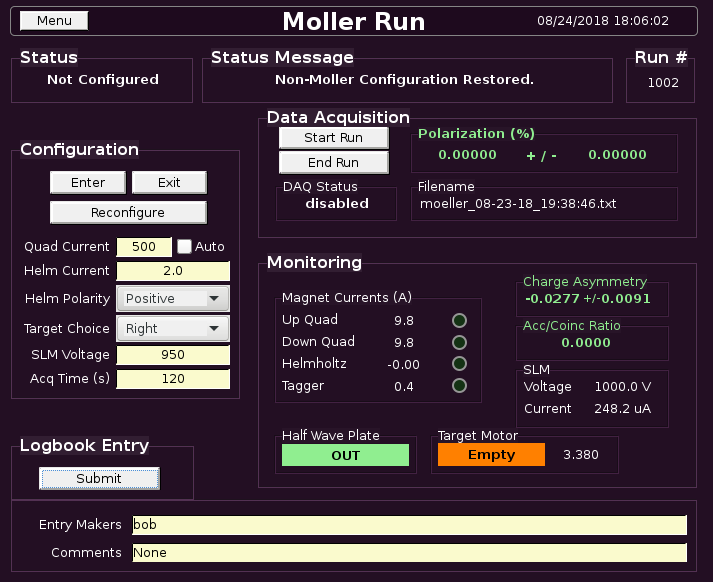
\includegraphics[width=11cm]{pics/unconfig}
    \caption{The user interface for shift workers for operating a M{\o}ller run is divided into {\em Status}, {\em Configuration}, {\em Data Acquisition}, {\em Monitoring}, and {\em Logbook} sections.  In this screenshot, the M{\o}ller system is not configured, according to the {\em Status} section, i.e. the setup is for non-M{\o}ller beam delivery.\label{fig:unconfig}}
\end{figure}

\newpage

\section{Hardware Settings}
The standard hardware settings, as of 2022, for a M{\o}ller run are shown in Table~\ref{tab:pars}.  These are displayed in the {\em Configuration} section of Figure~\ref{fig:unconfig} and will be used to automatically configure all hardware during the procedure in Section \ref{sec:user}.  It is the responsibility of the operator to ensure that the settings in the {\em Configuration} section are the desired ones before entering the M{\o}ller setup.  In case of any uncertainty, or inconsistency with parameters in this table, check with the beamline and/or slow controls expert.
\begin{table}[htbp]\centering
    \begin{tabular}{ll}\toprule[1.5pt]
        SLM Voltage & 1850 V \\
        Collimator Position & Blank \\
        Target Position & Left or Right \\
        Helmholtz Current & $\pm$3.5 A \\
        \cmidrule[0.5pt]{1-2}
        \multicolumn{2}{c}{Quadrupole Current} \\
        10.7 GeV & $\sim$3145 A (*)\\
        6.4 GeV & $\sim$1350 A (*)\\
        \bottomrule[1.5pt]
    \end{tabular}
    \caption{Standard hardware parameter values for the M{\o}ller setup as of 2022.  Live, measured values are shown in the {\em Monitoring} section in Figure~\ref{fig:unconfig}. {\em (*) Note, if ``Auto'' is selected for the quadrupoles in the ``Configuration'' section of Figure \ref{fig:unconfig}, the quadrupole currents will be set automatically based on the beam energy dependence in Figure \ref{fig:quadenergy}}.\label{tab:pars}}
\end{table}

\section{Quality Requirements}\label{sec:quality}
The requirements to be maintained during a M{\o}ller run, and the resulting desired error on the polarization measurement are shown in Table~\ref{tab:reqs}.  It is the responsibility of the operator to monitor these quantities to ensure a successful polarization measurement.
\begin{table}[htbp]\centering
    \begin{tabular}{ll}\toprule[1.5pt]
        2C21 BPM Current & $\sim$15 nA\\
        Beam Charge Asymmetry & $<0.2\%$ (typical $\sim 0.1\%$)\\
        Accidental/Coincidence Ratio & $<0.1$ (typical $\sim 0.05$)\\
        Final Beam Polarization Error & $<1.5\%$ (absolute)\\
        \bottomrule[1.5pt]
    \end{tabular}
    \caption{Standard quality conditions required for a M{\o}ller run.  Live values are shown in the {\em Monitoring} and {\em Data Acquisition} sections in Figure~\ref{fig:unconfig}.  Note, beam polarization error depends on statistics and should gradually decrease during the run.\label{tab:reqs}}
\end{table}

\newpage

\section{Standard Procedures}\label{sec:user}
Before starting the M{\o}ller procedure, confirm that Hall B orbit locks are off and our Halo and BOM FSD are masked.
\subsection{Procedure Summary}
The procedure for the operator with the interface in Figure~\ref{fig:unconfig} can be summarized in the following steps, and more details are shown on the next section.
\begin{enumerate}
\vspace{-4mm}\item {\bf Request No Beam:}  ask MCC to take beam away for a configuration change
\vspace{-4mm}\item {\bf Configure:}  ensure the Configuration section is set as desired
\vspace{-4mm}\item {\bf Enter:} click {\em Enter} in the Configuration section and wait for success status
\vspace{-4mm}\item {\bf Request 15 nA:} ask MCC to resume beam delivery at 15 nA for M{\o}ller runs
\vspace{-4mm}\item {\bf Start Run:} click {\em Start Run} in the DAQ section
\vspace{-4mm}\item {\bf Monitor:} monitor the critical parameters
\vspace{-4mm}\item {\bf End Run:} click {\em End Run} in the DAQ section
\vspace{-4mm}\item {\bf Log Entry:} click {\em Submit} in the Logbook Entry section 
\vspace{-4mm}\item {\bf Request No Beam:} ask MCC to take beam away for a configuration change
\vspace{-4mm}\item {\bf Reconfigure:} (Optional)
\vspace{-4mm}\item {\bf Exit:} click {\em Exit} in the Configuration section and wait for success status
\end{enumerate}

\subsection{Procedure Details}
\begin{enumerate}
    \item {\bf Request No Beam:}  ask MCC to take beam away while you configure the M{\o}ller system
    \item {\bf Configure:}  ensure the Configuration section of Fig.~\ref{fig:unconfig} is set as desired
        \subitem
        See Table~\ref{tab:pars} for standard values.  Contact the Run Coordinator if uncertain.
\item {\bf Enter:} click {\em Enter} in the Configuration section and wait for success status
    \subitem This will configure the system for a M{\o}ller run by initiating a sequence of actions and provide corresponding feedback in the status portion of the screen.  This includes turning off all appropriate detectors' high voltage, inserting the blank collimator, energizing the quadrupoles and Helmholtz magnets, and inserting the M{\o}ller target.  Success will result in ``Moller Configuration Ready'' in the status message.
\item {\bf Request 15 nA:} \label{step:beam} ask MCC to resume beam delivery at 15 nA for M{\o}ller runs
\item {\bf Start:} \label{step:start} once beam is stable, click {\em Start Run} in the DAQ section
    \subitem This will initiate a new M{\o}ller run, including zeroing any accumulated data, opening a new data file, incrementing the run number, and starting data acquisition.
\item {\bf Monitor:} monitor the critical quality parameters
    \subitem This is left to the operator, described in Table~\ref{tab:reqs}, with possible actions in Section~\ref{sec:knobs}.  Of particular importance are beam charge asymmetry below 0.2\% and accidental ratio of less than 0.1, although ideally about half that.  {\em If you cannot achieve the quality requirements, contact the Run Coordinator.}
\item {\bf End:} click {\em End Run} in the DAQ section
    \subitem At this point you should have achieved the desired polarization error of $1.5\%$ (see Table~\ref{tab:reqs}), or just need to stop the current run and start a new one (in which case, go to Step \#\ref{step:start}).
\item {\bf Log Entry}: click {\em Submit} in the Logbook Entry section if the run was successful. 
    \subitem This will submit a standardized, searchable log entry to HBLOG with a table summarizing the results and an attached data file, and requires filling the Entry Makers and Comments fields.  {\em Note, if you want to log any screenshots associated with this M{\o}ller run, then you should navigate to this log entry and upload them as comments}.
    \subitem Note, at this point you can start another run with the same configuration by going to Step \#\ref{step:start}.
\item {\bf Request No Beam:} ask MCC to take beam away before changing the M{\o}ller configuration
\item {\bf Reconfigure:}  (Optional)  At this point you may reconfigure the system (e.g. change the Helmholtz polarity or switch to a different target, and then click {\em Reconfigure}, or just ask MCC for a change in the Half-Wave Plate) and then start another run (go to Step \#\ref{step:beam}).
\item {\bf Exit}: click {\em Exit} in the Configuration section and wait for success status
    \subitem  This will restore the non-M{\o}ller configuration by turning off the quadrupoles and Helmholtz and retracting the M{\o}ller target.  {\em Note, this will not restore any detector high voltage (except the SLM) nor move the collimator}. 
\end{enumerate}

\newpage
\section{Quality Requirements}\label{sec:knobs}

If quality requirements are not satisfied (accidental rate and beam charge asymmetry), first check whether our hardware settings are as expected by comparing to the parameters earlier in this document and also to recent satisfactory M{\o}ller runs in the logbook.  The following subsections contain information on the quality measurements and the main parameters that can affect them.  Consult with the Run Coordinator and/or beamline expert for advice on tuning these parameters, and compare their values with previous M{\o}ller runs.

\subsection{Run Duration}
At 10 GeV, with our 2018 hardware configuration, the normal run duration to achieve 1.5\% absolute error on the polarization is about 30 minutes of continuous beam.  Interruptions to beam delivery, e.g. trips, will of course increase the necessary run time.  Much longer than normal run duration to achieve 1.5\% can be indicative of excessive accidentals or beam charge asymmetry.

\subsection{Beam Charge Asymmetry}
Beam charge asymmetry is measured by a Synchrotron Light Monitor fed to a Struck scaler latching on the heliticy signals.  The SLM is located a few meters upstream of, and {\em completely independent of}, the rest or our M{\o}ller system.  Beam Charge asymmetry is affected primarily by beam characteristics from the injector and accelerator.  There can be some effect from quality of the SLM performance, e.g. if voltage is far too high and the SLM is saturated, but this should generally never be the case for the normal operator.

Note that beam charge asymmetry updates with the same period as our Moller acquisition time, i.e. if the acquisition time is set at 60 seconds, beam charge asymmetry will only update once per minute.

If the beam charge asymmetry is too high, the parameters that can be considered are:
\begin{itemize}
\vspace{-4mm}\item Beam position (BPM and harp scans)
\vspace{-4mm}\item Beam profile (harp scans)
\vspace{-4mm}\item Injector slit setting
\vspace{-4mm}\item Injector attenuator settings
\end{itemize}

\subsection{Accidentals}
The accidental-coincidence ratio is measured by M{\o}ller Left/Right PMTs, downstream of the target and quadrupoles, and is independent of the helicity signals.  Excessive accidentals can be caused by beam quality issues, e.g. bleedthrough from other halls, or non-optimal settings of our M{\o}ller system.  Parameters that can be considered for adjustment include the same beam quality parameters in the previous section, and with the addition of our M{\o}ller configuration, e.g. Left/Right PMT voltages, malfunctioning quadrupoles, or very miscalibrated target position.

\begin{figure}[htbp]\centering
    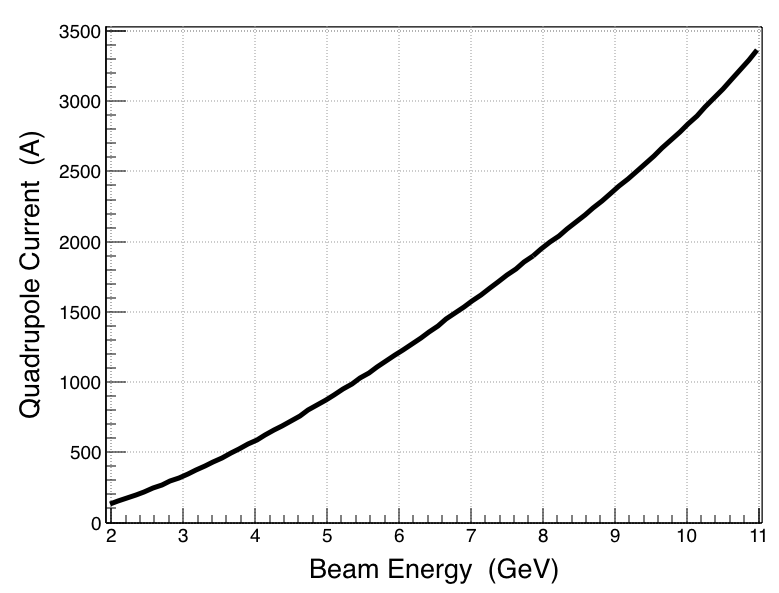
\includegraphics[width=14cm]{pics/moller_quad_current}
    \caption{The calculated optimal quadrupole current as a function of beam energy.  This is the function used if the {\em Auto} checkbox is selected in the {\em Configuration} section of Figure \ref{fig:unconfig} when entering or reconfiguring the Moller setup.\label{fig:quadenergy}}
\end{figure}

\end{document}

